\chapter{Sum-Product Networks}
\label{cap:spn}

In this chapter, we review some literature about SPNs. We will begin by introducing the definition and fundamental concepts of SPNs (Section \ref{sec:spn:fundamentals}) and showing how an SPN is evaluated (Section \ref{sec:spn:evaluation}). Then, we will leverage the relation between SPNs and mixture models, and, particularly, the relation between GSPNs and GMMs (Section \ref{sec:spn:trees}). Next, we will show how SPNs are learned from data (Section \ref{sec:spn:learning}). Finally, we will review the literature on performing Maximum-A-Posteriori inference in SPNs, which is equivalent to finding a global maximum (Section \ref{sec:spn:map}).

Assuming the reader's familiarity with standard definitions of graph theory \citep{Bondy2008}, we proceed to use them throughout this work without further elaboration.

\section{Fundamentals}
\label{sec:spn:fundamentals}

We define the \textbf{scope} of a Sum-Product Network as the set of variables that appear in it, and we define \textbf{Sum-Product Network} (SPN) recursively \citep{Gens2013}.

\begin{definition}[Sum-Product Network]
  A Sum-Product Network is defined as follows:

  \begin{itemize}
    \item Any tractable univariate distribution is an SPN.
    \item Any product of SPNs with disjoint scopes is an SPN.
    \item Any weighted sum of SPNs with the same scope and nonnegative weights adding up to $1$ is an SPN.
    \item Nothing else is an SPN.
  \end{itemize}
\end{definition}

SPNs are commonly represented as rooted directed acyclic graphs with three types of nodes:

\begin{itemize}
  \item A univariate distribution is represented as a leaf.
  \item A product of SPNs is represented as an internal product node (denoted by $\times$) with nonweighted edges to the SPNs which it multiplies.
  \item A weighted sum of SPNs is represented as an internal sum node (denoted by $+$) with weighted edges to the SPNs which it sums.
\end{itemize}

The recursive construction of an SPN, as defined above, ensures that every node in the network readily represents a probability distribution over its scope. Specifically, leaves are distributions by definition, product nodes represent distributions under the assumption of independence among their children distributions, and sum nodes represent mixture distributions \citep{Peharz2015}.

\begin{figure}
  \begin{minipage}{0.5\textwidth}
    \centering
    \scalebox{1}{
      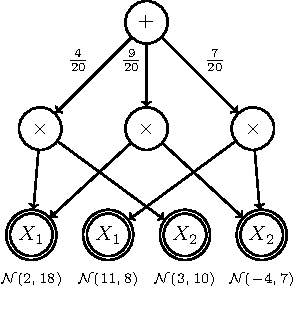
\includegraphics{figures/gspn-b.pdf}
    }

    (a)
  \end{minipage}\begin{minipage}{0.5\textwidth}
    \centering
    \scalebox{0.82}{
      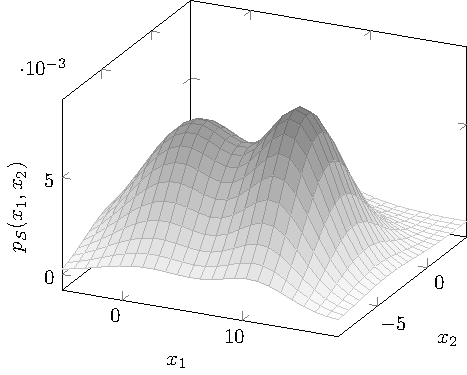
\includegraphics{figures/gspn-c.pdf}
    }

    (b)
  \end{minipage}

  \caption[A GSPN and a plot of its PDF]{
    \textbf{(a)} A SPN $\mathcal{S}$ with Gaussian leaves.
    \textbf{(b)} Plot of the PDF of the distribution $\mathcal{S}$.
  }
  \label{fig:gspn}
\end{figure}

SPNs can be constructed using discrete, continuous, or hybrid (mixed) variables. Although many studies have been conducted on SPNs based on categorical random variables, there are many real-world applications that are better suited to continuous variables \citep{Jaini2016}. In this study, we concentrate on SPNs that use continuous RVs (learned from continuous data), particularly SPNs with univariate Gaussian distributions at their leaves. We refer to these networks as \textbf{Gaussian Sum-Product Networks} (GSPNs).

\begin{definition}[Gaussian Sum-Product Network]
  A Gaussian Sum-Product Network is a Sum-Product Network with only univariate Gaussian distributions at their leaves.
\end{definition}

\noindent Figure \ref{fig:gspn}(a) displays an example of a GSPN, and \ref{fig:gspn}(b) depicts its probability density function. Although marginal inference works the same way for discrete and continuous SPNs (except that discrete SPNs compute probability masses, whereas continuous SPNs compute densities), certain algorithms that operate on discrete SPNs may not function with continuous SPNs and vice versa.

\section{Inference in SPNs}
\label{sec:spn:evaluation}

The process of performing reasoning in probabilistic models is called \textbf{inference}. SPNs allow performing marginal inference and conditional inference in linear time in the size of the network.

Given an SPN $\mathcal{S}$, we denote its probability distribution function as $\mathcal{S}(\cdot)$. To perform marginal inference, that is, to compute the probability of a valuation $\mathbf{x}$ of RVs $\mathbf{X}$ in the SPN $\mathcal{S}$, $\mathcal{S}(\mathbf{X} = \mathbf{x})$, we traverse the graph in reverse topological order. For a node $u$ in an SPN $\mathcal{S}$, let $u(\mathbf{x})$ denote the value of the node $u$ in the SPN given the valuation $\mathbf{X} = \mathbf{x}$ restricted to the RVs in the scope of $u$ and let $\ch(u)$ denote the children of $u$ in the DAG. Then,

\begin{enumerate}
  \item If $u$ is a leaf, $u(x)$ is the density of $x$ of its corresponding univariate distribution over $X$.
  \item If $u$ is a product node, $u(\mathbf{x})$ is the product of its children:

        \begin{equation}
          u(\mathbf{x}) = \prod_{v \in \ch(u)} v(\mathbf{x}) \, .
        \end{equation}
  \item If $u$ is a sum node, $u(\mathbf{x})$ is the weighted sum of its children:

        \begin{equation}
          u(\mathbf{x}) = \sum_{v \in \ch(u)} w(u, v)v(\mathbf{x}) \, .
        \end{equation}
\end{enumerate}

\noindent The distribution of an SPN is the distribution of its root node. A pseudocode of marginal inference in an SPN is given in Algorithm \ref{alg:inference}.

\begin{algorithm}[h]
  \caption{Marginal inference in SPNs}
  \label{alg:inference}
  \begin{algorithmic}
    \Input{an SPN $\mathcal{S}$ over $\mathbf{X}$ and an assignment $\mathbf{x}$}
    \Output{$\mathcal{S}(\mathbf{X} = \mathbf{x})$}
  \end{algorithmic}
  \begin{algorithmic}[1]
    \LineComment{Let $V$ be a mapping from SPN nodes to values, initially empty.}
    \ForAll{node $u$ of $\mathcal{S}$ in reverse topological order}
    \If{$u$ is a leaf}
    \State $V_u \gets u(\mathbf{x})$
    \ElsIf{$u$ is a product node}
    \State $V_u \gets \prod_{v \in \ch(u)} V_v$
    \ElsIf{$u$ is a sum node}
    \State $V_u \gets \sum_{v \in \ch(u)} w_v V_v$
    \EndIf
    \EndFor
    \State \Return{$V_u$}
  \end{algorithmic}
\end{algorithm}

\begin{example}
  Let $\mathcal{S}$ be the GSPN represented in Figure \ref{fig:gspn}. Then

  \begin{multline}
    \mathcal{S}(x_1, x_2) = \frac{4}{20} \mathcal{N}(x_1; 2, 18) \mathcal{N}(x_2; 3, 10) + \frac{9}{20} \mathcal{N}(x_1; 2, 18) \mathcal{N}(x_2; -4, 7) \\
    + \frac{7}{20} \mathcal{N}(x_1; 11, 8) \mathcal{N}(x_2; -4, 7),
    \label{eq:spninference}
  \end{multline}

  \noindent where $\mathcal{N}(x; \mu, \sigma^2)$ is a shorthand to represent the density of $x$ in the Gaussian distribution $\mathcal{N}(\mu, \sigma^2)$. If $x_1 = 11$ and $x_2 = -4$, then

  \begin{eqnarray*}
    \mathcal{S}(x_1, x_2) & \approx & \frac{4}{20} \times 0.00991 \times 0.01089 + \frac{9}{20} \times 0.00991 \times 0.15079 \\
    & & + \frac{7}{20} \times 0.14105 \times 0.15079 \\
    & \approx & 0.00814 \, .
  \end{eqnarray*}

  The inference process is illustrated in Figure \ref{fig:spninference}.
\end{example}

\begin{figure}
  \centering
  \scalebox{0.9}{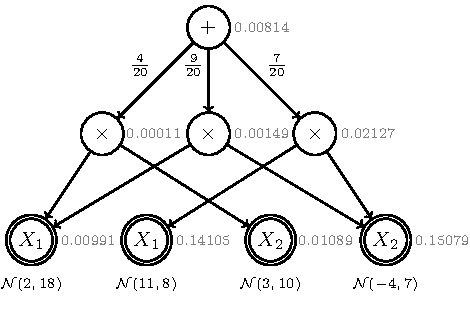
\includegraphics{figures/spninference.pdf}}

  \caption[Marginal inference in a GSPN]{Inference of $\mathcal{S}(11, -4)$ in the SPN represented in Figure \ref{fig:gspn}. The approximate values of the nodes, computed in a bottom-up fashion, are on the right side of each node.}
  \label{fig:spninference}
\end{figure}

\section{SPNs as mixture models}
\label{sec:spn:trees}

\citet{Zhao2015} showed that any SPN is equivalent to a mixture of trees where each tree corresponds to a product of univariate distributions. Given an SPN $\mathcal{S}$ over $X_1, \cdots, X_n$, let $\mathcal{T} = (V_\mathcal{T}, E_\mathcal{T})$ be a subgraph of $\mathcal{S}$. $\mathcal{T}$ is called an \textbf{induced tree}\footnote{This notion has been used in the literature under different terms, e.g. \emph{induced tree} by \citet{Zhao2015}, \emph{parse tree} by \citet{Mei2017}, \emph{complete subnetwork} by \citet{Desana2016}, \emph{complete sub-circuit} by \citet{Chan2006, Dennis2015}.} from $\mathcal{S}$ if it can be constructed recursively, starting from the root node and then including all children of product nodes and exactly one child of sum nodes (with the corresponding edges). As proved by \citet[Theorems 1 and 2]{Zhao2015}, an induced tree $\mathcal{T}$ is an SPN, therefore $\mathcal{T}(\mathbf{X})$ represents a probability distribution. The density function of such distribution is given by:

\begin{equation}
  \mathcal{T}(\mathbf{x}) = \prod_{(u, v) \in E_\mathcal{T}} w(u, v) \prod_{j=1}^{n} T_j(x_j) \, ,
  \label{eq:inducedtree}
\end{equation}

\noindent where $w(u, v)$ is the weight of the edge $(u, v) \in E_\mathcal{T}$ if $u$ is a sum node or $1$ if $u$ is a product node; $T_j(X_j)$ is the probability distribution of a leaf of $\mathcal{T}$ ($\mathcal{T}$ contains $n$ leaves, one for each variable).

Let $\tau_\mathcal{S}$ denote the number of unique induced trees from $\mathcal{S}$, namely, its \textbf{network cardinality}, and $\mathcal{T}^i$ denote the $i$-th unique induced tree of $\mathcal{S}$. Then \citep[Theorem 4]{Zhao2015},

\begin{equation}
  \mathcal{S}(\mathbf{x}) = \sum_{i=1}^{\tau_\mathcal{S}} \mathcal{T}^i(\mathbf{x}) \, .
  \label{eq:mixture}
\end{equation}

\noindent This result is illustrated in Figure \ref{fig:inducedtrees}. The network cardinality of $\mathcal{S}$ depends on its structure and is exponential in the height of the SPN.

\begin{figure}
  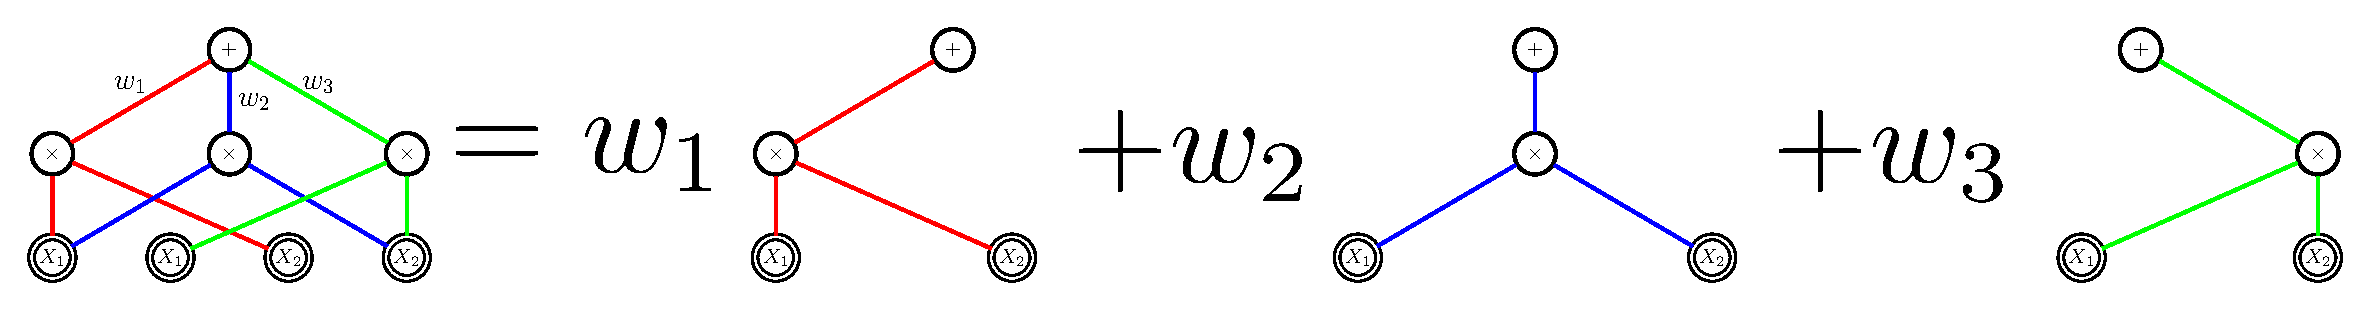
\includegraphics[width=\textwidth]{figures/inducedtrees.pdf}

  \caption[SPN as a mixture of induced trees]{An SPN as a mixture of induced trees. Source: \citet{Zhao2015}.}
  \label{fig:inducedtrees}
\end{figure}

\vspace{1em}

Given an SPN $\mathcal{S}$, from equations \ref{eq:inducedtree} and \ref{eq:mixture} we have:

\begin{equation}
  \label{eq:inducedtree_i}
  \mathcal{S}(\mathbf{x}) = \sum_{i=1}^{\tau_\mathcal{S}} w_i T^i(\textbf{x}) \, ,
\end{equation}

\noindent where $w_i := \prod_{(u, v) \in E_{\mathcal{T}_i}} w(u, v)$ and $T^i(\mathbf{x}) := \prod_{j=1}^n T^i_j(x_j)$ for all $i = 1, \cdots, \tau_\mathcal{S}$ (we are just splitting $\mathcal{T}_i$).

Let $Z$ be the latent variable that corresponds to the mixture, i.e., $\mathcal{S}(\mathbf{x} \mid z) = T^z(\textbf{x})$, and let $x_k, \cdots, x_l$ be values of RVs in $\mathbf{X}$. Then, for all $z \sim Z$,

\begin{eqnarray}
  \mathcal{S}(x_k, \cdots, x_l \mid z) & = & T^z(x_k, \cdots, x_l) \\
  & = & \prod_{j=1}^n T^z_j(x_k, \cdots, x_l) \\
  & = & T^z_k(x_k) \cdots T^z_l(x_l) \\
  & = & \mathcal{S}(x_k \mid z) \cdots \mathcal{S}(x_l \mid z) \, ,
\end{eqnarray}

\noindent which implies that the (observable) variables are independent given the mixture.

\vspace{1em}

If $\mathcal{S}$ is a GSPN, then $T^z(\mathbf{X})$ is a PDF formed by the product of the PDFs of independent Gaussian RVs. Thus, $T^z(\mathbf{X})$ is a multivariate Gaussian distribution with a diagonal covariance matrix. Therefore, a GSPN represents a GMM, where in each component the variables are uncorrelated.

However, GSPNs have an exponential network cardinality (with respect to the height of the network); therefore, they represent GMMs with a huge number of components. Despite the components share some parameters, this makes GSPNs much more expressive than typical learned GMMs while still remaining computationally tractable.

\section{Learning SPNs}
\label{sec:spn:learning}

SPNs are typically learned from data, and there exist various methods to accomplish this \citep{Peharz2015}. While recently, a variety of random methods that waive the necessity of structure learning have gained popularity \citep{Peharz2020, Geh2021}, in this section, we will focus on reviewing the most classical one -- LearnSPN. Our aim is not to delve too deeply into the topic of learning SPNs, but rather to gain a better understanding of the structure of the SPNs used in our experiments and the influence of learning parameters on these SPNs.

\textbf{LearnSPN}, the most classical schema used to learn SPNs \citep{Gens2013}, operates through a top-down divide-and-conquer approach that can learn both the structure (the underlying graph) and the parameters (weights and distributions at the leaves) of an SPN. To achieve this, it recursively splits the training set matrix into matrices with fewer instances or fewer variables, as shown in Figure \ref{fig:learnspn}. A high-level summary of the LearnSPN algorithm is presented in Algorithm \ref{alg:learnspn}.

\begin{figure}
  \centering
  \scalebox{0.3}{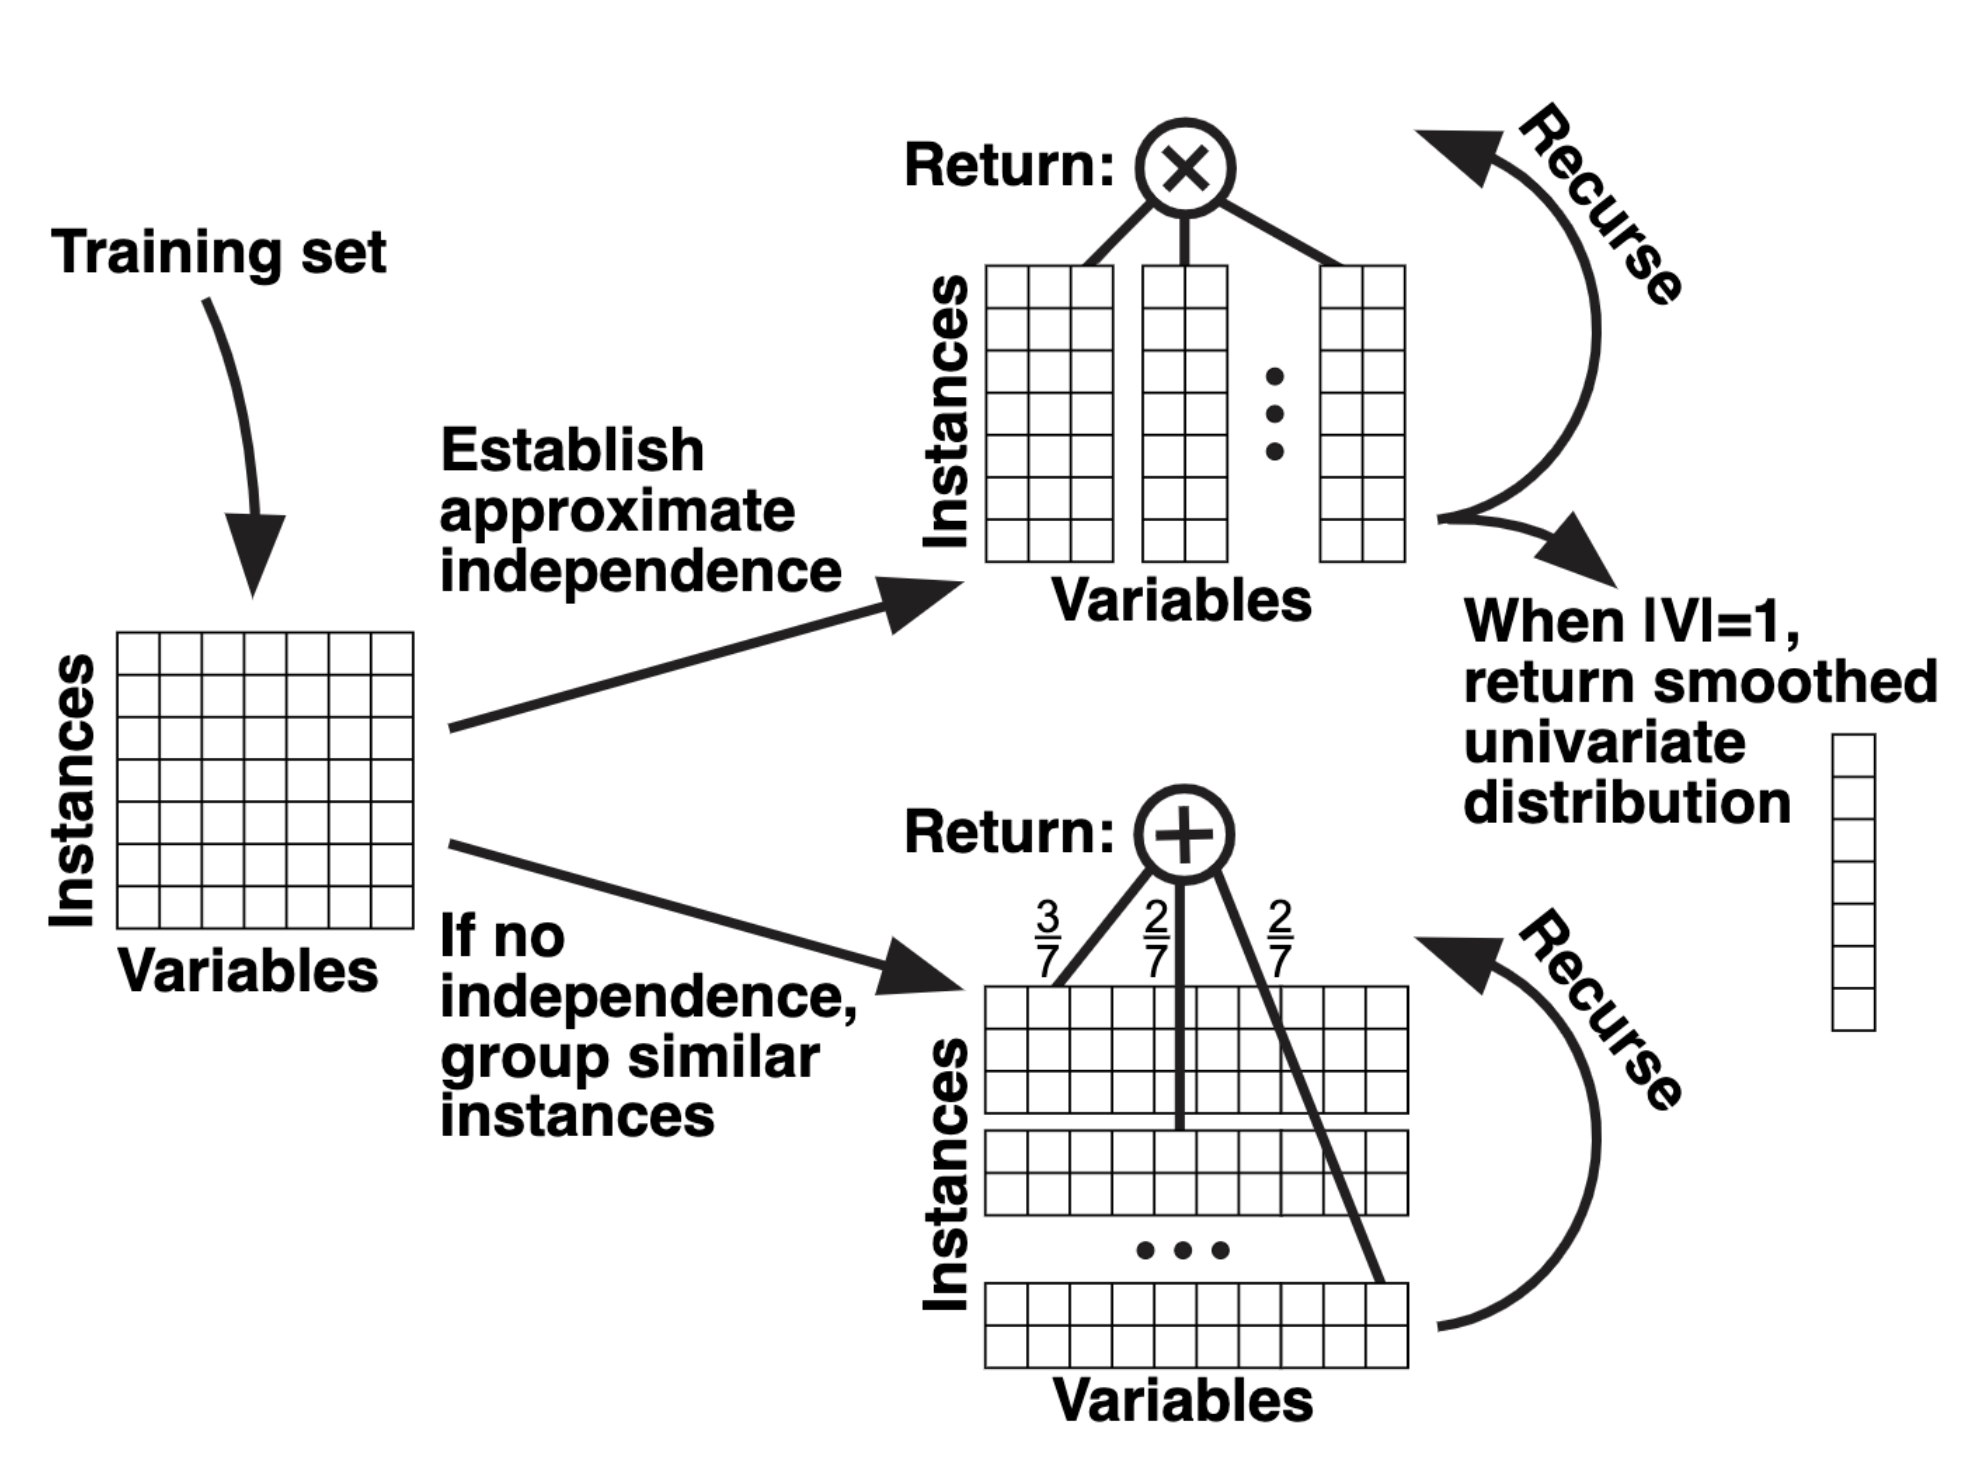
\includegraphics{figures/learnspn.png}}

  \caption[LearnSPN schema]{Illustration of LearnSPN algorithm. Source: \citet{Gens2013}.}
  \label{fig:learnspn}
\end{figure}

\begin{algorithm}[h]
  \caption{LearnSPN schema}
  \label{alg:learnspn}
  \begin{algorithmic}
    \Input{set of instances $D$ and set of variables $V$}
    \Output{an SPN representing a distribution over $V$ learned from $D$}
  \end{algorithmic}
  \begin{algorithmic}[1]
    \If{$|V| = 1$}
    \State \Return{univariate distribution estimated from the variable's values in $D$}
    \Else
    \LineComment{Try to partition $V$ into approximately independent subsets $V_j$.} \label{alg:learnspn:prod}
    \If{partition is successful}
    \State \Return{product node pointing to all $\textrm{LearnSPN}(D, V_j)$}
    \Else
    \LineComment{Partition $D$ into subsets of similar instances $D_i$.} \label{alg:learnspn:sum}
    \State \Return{sum node pointing to all $\textrm{LearnSPN}(D_i, V)$ with weights $\frac{|D_i|}{|D|}$}
    \EndIf
    \EndIf
  \end{algorithmic}
\end{algorithm}

The specificities for partitioning a variable set $V$ into approximately independent subsets $V_j$ (line \ref{alg:learnspn:prod}) and partitioning a dataset $D$ into subsets of similar instances $D_i$ (line \ref{alg:learnspn:sum}) were intentionally left vague by \citet{Gens2013}, making LearnSPN more of a schema than a single algorithm.

It is important to highlight that LearnSPN exclusively learns tree-shaped SPNs. Consequently, the resulting structures tend to be larger than if they were not constrained to trees. Furthermore, this implies that there is likely a considerable number of leaves associated with each variable.

There are different approaches to accomplish partitioning the dataset. One common method for finding approximately independent subsets of variables is the G-test \citep{Gens2013}. However, different implementations may employ different independence tests. For instance, the open-source library SPFlow \citep{Molina2019SPFlow} utilizes the Randomized Dependence Coefficient \citep{Lopes-Paz2013} as its default independence test.

To split instances, clustering methods can be employed, such as $k$-means \citep{MacQueen1967} and GMM clustering. Each of these methods requires specific hyperparameters. In LearnSPN implementations, it is typical to specify a threshold for determining variable independence, a minimum number of instances for partitioning, a desired number of clusters, and, in the case of learning GSPNs, a minimum variance for the Gaussian distributions in the leaves to prevent the learning of degenerate GSPNs.

The choice of hyperparameters has a significant impact on the size of learned SPNs.

\section{MAP inference}
\label{sec:spn:map}

SPNs are often built to solve structured prediction problems, where a solution is found by performing \textbf{Maximum-A-Posteriori} (MAP) inference in the model. MAP inference aims to find the most probable values for a set of RVs according to a probability distribution, and it is closely related to finding a global maximum in SPNs.

\begin{definition}[MAP Inference]
  Given a probability density function\footnote{We are assuming continuous RVs, but in the case of discrete RVs the definition is similar but uses a probability mass function instead of a probability density function.} $p(\mathbf{X})$, disjoint sets $\mathbf{X}^q$, $\mathbf{X}^0$, $\mathbf{X}^m$ such that $\mathbf{X} = \mathbf{X}^q \cup \mathbf{X}^0 \cup \mathbf{X}^m$, and an evidence $\mathbf{x}^0$ on $\mathbf{X}^0$, MAP inference consists of finding the most probable configuration for $\mathbf{X}^^q$ given $\mathbf{x}^0$ and ignoring (marginalizing) the RVs in $\mathbf{X}^m$, that is:

  \begin{equation}
    \label{eq:map}
    \MAP\left(p, \mathbf{X}^q, \mathbf{x}^0, \mathbf{X}^m\right) := \argmax_{\mathbf{x}^q \in \mathbb{R}^{|\mathbf{X}^q|}}{p\left(\mathbf{x}^q \mid \mathbf{x}^0\right)} \, .
  \end{equation}
\end{definition}

MAP inference is a generalization of Most Probable Explanation (MPE) inference, which consists in finding the most probable configuration for a set of RVs $\mathbf{X}^q$ given an evidence $\mathbf{x}^0$ (without a set of RVs to marginalize), and is inherently harder than it in classical probabilistic graphical models (PGMs) like Bayesian Networks and Markov Networks \citep{Park2004}.

Equation \ref{eq:map} implies that:

\begin{eqnarray}
  \MAP\left(p, \mathbf{X}^q, \mathbf{x}^0, \mathbf{X}^m\right) & = & \argmax_{\mathbf{x}^q \in \mathbb{R}^{|\mathbf{X}^q|}}{p\left(\mathbf{x}^q, \mathbf{x}^0\right)} \\
  & = & \argmax_{\mathbf{x}^q \in \mathbb{R}^{|\mathbf{X}^q|}}{\int_\mathbb{R} \cdots \int_\mathbb{R} p\left(\mathbf{x}^q, \mathbf{x}^0, x^m_1, \cdots, x^m_k\right) dx^m_1 \cdots dx^m_k} \, .
\end{eqnarray}

The valuation $\MAP(\cdot)$ is named \textbf{MAP assignment} and the conditional probability $p(\MAP(\cdot) \mid \mathbf{x}^0)$ is named \textbf{MAP value}. In this work, we refer to the problem of performing MAP inference as \textbf{MAP problem}.

\vspace{1em}

Although marginal and conditional inference take linear time in SPNs, MAP inference is computationally difficult. In fact, it is proven to be $\mathcal{NP}$-Hard in discrete SPNs; distinct proofs are found in \citep{Peharz2015}, \citep{Peharz2016} and \citep{Conaty2017}. Moreover, \citet{Conaty2017} proved the non-approximability of MAP inference within a sublinear factor in discrete SPNs of height 2, as well as the non-approximability within any factor $2^{f(m)}$ for any sublinear function $f$ of the input size $m$ in discrete SPNs of height $\geq 3$, even if there is no evidence and if their structure is a tree. Their results are summarized in Table \ref{tab:mapcomplexity}.

\begin{table}
  \centering

  \begin{tabular}{ccc}
    \toprule
    \bfseries Height & \bfseries Lower bound & \bfseries Upper bound \\ \midrule
    $1$              & $1$                   & $1$                   \\
    $2$              & $(m-1)^\epsilon$      & $m-1$                 \\
    $\geq 3$         & $2^{s^\epsilon}$      & $2^s$                 \\
    \bottomrule
  \end{tabular}

  \caption[Lower and upper bounds on the approximation threshold for a polynomial-time algorithm for MAP inference in discrete SPNs]{Lower and upper bounds on the approximation threshold for a polynomial-time algorithm for MAP inference in discrete SPNs: $s$ denotes the size of the instance, $m$ is the number of internal nodes, $\epsilon$ is a non-negative number less than $1$. Source: \citet{Conaty2017}.}
  \label{tab:mapcomplexity}
\end{table}

\subsection{Reduction from MAP to MAX}
\vspace{1em}

MAP inference splits the set of RVs $\mathbf{X}$ in three parts $\mathbf{X}^q$, $\mathbf{X}^0$, $\mathbf{X}^m$ such that $\mathbf{X} = \mathbf{X}^q \cup \mathbf{X}^0 \cup \mathbf{X}^m$. \citet{Mei2017} proved that every MAP problem can be reduced to a special case of MAP inference without evidence and RVs to marginalize ($\mathbf{X}^0 = \emptyset$, $\mathbf{X}^m = \emptyset$) in linear time in the size of the SPN. Formally, this reduced problem, which they called MAX inference, consists in computing:

\begin{equation}
  \MAX(p) := \argmax_{\mathbf{x}} p(\textbf{x}) \, ,
\end{equation}

\noindent that is, to find the global maximum of a PDF.

The transformation of a MAP problem to a MAX problem in linear time implies that any efficient algorithm for solving MAX inference can be used to efficiently solve MAP inference.

Given a MAP problem $\mathbf{X}^q, \mathbf{x}^0, \mathbf{X}^m$ over an SPN $\mathcal{S}$, the MAP2MAX algorithm developed by \citet{Mei2017} returns a new SPN $\mathcal{S}'$ over $\mathbf{X}^q$ such that $\mathcal{S}'(\mathbf{x}^q) = \mathcal{S}(\mathbf{x}^q, \mathbf{x}^0)$ for all $\mathbf{x}^q \in \mathbb{R}^{|\mathbf{X}^q|}$, which implies $\MAX(\mathcal{S}') = \MAP(\mathcal{S}, \mathbf{X}^q, \mathbf{x}^0, \mathbf{X}^m)$. A pseudocode is given in Algorithm \ref{alg:map2max}. It is slightly modified from the one in the original paper because \citet{Mei2017} considers SPNs with RV indicators at their leaves.

\begin{algorithm}[h]
  \caption{MAP2MAX}
  \label{alg:map2max}
  \begin{algorithmic}
    \Input{an SPN $\mathcal{S}$ over $\mathbf{X}$, an evidence $\mathbf{x}^0$, and a set $\mathbf{X^m}$ of RVs to marginalize}
    \Output{an SPN $\mathcal{S'}$ over $\mathbf{X}^q$ such that $\mathcal{S}'(\mathbf{x}^q) = \mathcal{S}(\mathbf{x}^q, \mathbf{x}^0)$}
  \end{algorithmic}
  \begin{algorithmic}[1]
    \LineComment Let $A$ be an auxiliary mapping from SPN nodes to real values.
    \ForAll{node $u$ of $\mathcal{S}$ in reverse topological order}
    \If{$u$ is a leaf with scope $X_i$}
    \If{$X_i \in \mathbf{X}^e$}
    \State $A_u \gets u(x^e_i)$
    \Else
    \State $A_u \gets -\infty$
    \EndIf
    \ElsIf{$u$ is a product node}
    \State $A_u \gets \prod_{v \in \ch(u)} A_v$
    \ElsIf{$u$ is a sum node}
    \ForAll{$v \in \ch(u)$}
    \State $w(u, v) \gets w(u, v) A_v$
    \EndFor
    \If{$\scope(u) \subseteq \mathbf{X}^e \cup \mathbf{X}^m$}
    \State $A_u \gets \sum_{v \in \ch(u)} w(u, v)$
    \Else
    \State{$A_u \gets 1$}
    \EndIf
    \EndIf
    \EndFor
    \ForAll{node $u$ of $\mathcal{S}$}
    \If{$\scope(u) \subseteq \mathbf{X}^e \cup \mathbf{X}^m$}
    \LineComment{Remove $u$ and the arcs/weights associated with $u$.}
    \EndIf
    \EndFor
    \State \Return{$\mathcal{S}$}
  \end{algorithmic}
\end{algorithm}

To be precise, the SPN resulting from MAP2MAX algorithm is not ``normalized,'' as the weights of arcs from sum nodes do not necessarily add up to 1 and therefore the resulting probability distribution is not normalized. However, SPNs can be normalized efficiently in linear time, as shown by \citet{Peharz2015}, and the normalization simply divides densities by a constant, not affecting the semantic of the model and its modes.

Since MAP inference can be reduced to MAX in linear time, we will assume, without loss of generality, that MAP inference in SPNs is seeking the solution to the MAX problem, which consists in simply finding a global maximum of a given distribution.

\subsection{Approximation algorithms}
\label{sec:map:approximate}

Table \ref{tab:mapcomplexity} shows that MAP inference in SPNs is not only hard to perform exactly, but also hard to approximate. Since the introduction of SPNs, different approximation algorithms have been proposed; first Max-Product \citep{Poon2011}, and then adaptations such as ArgMax-Product \citep{Conaty2017} and K-Best Tree \citep{Mei2017}.

\vspace{1em}

\textbf{Max-Product} is a greedy algorithm that runs in linear time and consists of, given an SPN $\mathcal{S}$:

\begin{enumerate}
  \item Build a Max-Product Network $\mathcal{M}$ from $\mathcal{S}$ by replacing all sum nodes with $\max$ nodes (which selects the maximum values among its children). Replace each leaf with the global maximum of its distribution.
  \item Compute the values of all nodes in $\mathcal{M}$ by visiting all nodes starting from the leaves, similar to the process of performing marginal inference in an SPN as seen in Algorithm \ref{alg:inference}.
\end{enumerate}

The pseudocode for Max-Product is given in Algorithm \ref{alg:maxproduct}.

\begin{algorithm}[h]
  \caption{Max-Product}
  \label{alg:maxproduct}
  \begin{algorithmic}
    \Input{an SPN $\mathcal{S}$ over $\mathbf{X}$}
    \Output{a valuation $\mathbf{x}$ for $\mathbf{X}$ that is an approximation of $\argmax_{\mathbf{x}} \mathcal{S}(\textbf{x})$}
  \end{algorithmic}
  \begin{algorithmic}[1]
    \LineComment{For any node $u$, let $A_u$ denote a mapping from RVs to values (initially empty).}
    \ForAll{node $u$ of $\mathcal{S}$ in reverse topological order}
    \If{$u$ is a leaf over $X_i$}
    \State $A_u \gets \{X_i: \argmax_{x} u(x)\}$ \Comment{e.g. for $u \sim \mathcal{N}(\mu, \sigma^2)$, $\argmax_{x} u(x) = \mu$}
    \State $M_u \gets u(A_u[X_i])$
    \ElsIf{$u$ is a product node}
    \State $A_u \gets \cup_{v \in \ch(u)} A_v$
    \State $M_u \gets \prod_{v \in \ch(u)} V_v$
    \ElsIf{$u$ is a sum node}
    \State $v^* \gets \argmax_{v \in \ch(u)} w_v M_v$ \label{alg:maxproduct:sum}
    \State $A_u \gets A_{v^*}$
    \State $M_u \gets w_{v^*} M_{v^*}$
    \EndIf
    \EndFor
    \State \Return{$A_\textrm{root}$}
  \end{algorithmic}
\end{algorithm}

\begin{figure}
  \centering
  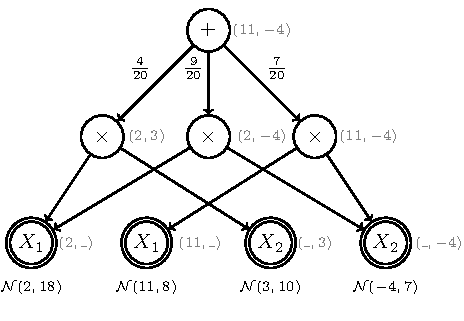
\includegraphics{figures/maxproduct.pdf}

  \caption[Illustration of Max-Product]{
    Max-Product algorithm in the GSPN shown in Figure \ref{fig:gspn}. On the right of each node $v$, the value of $\map_2(v)$ as computed by Max-Product. The algorithm outputs the configuration $X_1=11, X_2=-4$.
  }

  \label{fig:maxproduct}
\end{figure}

Figure \ref{fig:maxproduct} illustrates Max-Product algorithm finding a MAP assignment in the GSPN shown in Figure \ref{fig:gspn}.

This algorithm is called Best Tree by \citet{Mei2017} because it actually finds the induced tree of the SPN with the largest MAP value. \citet{Peharz2016} proved that it finds the exact solution of MAP inference in the subclass of selective SPNs\footnote{A sum node $u$ is \textbf{selective} if for all choices of weights $w$ and all possible $\mathbf{x}$ it holds that at most one child of $u$ is non-zero. An SPN is selective if all its sum nodes are selective.}, but that is not useful in the context of GSPNs which are not selective.

\vspace{1em}

\citet{Conaty2017} proposed a slightly modified version of Max-Product algorithm which they called \textbf{ArgMax-Product}. In the worst case scenario it achieves the same result of Max-Product, but reportedly perform significantly better in average. The idea is, for each sum node $u$, to compute the value of the sub-SPN rooted in $u$ for each of the possible MAP assignments obtained by its children. Instead of just choosing the maximum value of $w(u, v) A_v$ for all $v \in \ch(u)$ (line \ref{alg:maxproduct:sum}), it actually computes the entire value of $v$ for all the sets of values of RVs that arise from its children. The trade-off is complexity: ArgMax-Product does $|\ch(v)|$ bottom-up evaluations of the SPN on every sum node $v$ in the SPN, so it has quadratic time complexity.

\vspace{1em}

\citet{Mei2017} noted that, given an SPN $\mathcal{S}$, Max-Product algorithm finds the induced tree with the largest MAX value. Motivated by their empirical finding that in several cases the exact MAX solution is an induced tree with a large value, although not necessarily the largest, they proposed an algorithm to find the $K$ induced trees of $\mathcal{S}$ with the largest value --- namely, \textbf{K-Best Tree} (KBT). The algorithm is similar to Max-Product, but, instead of propagating up the maximum value from each node, it propagates the top $K$. The overall time complexity of KBT is $O(|\mathcal{S}| K \log{K})$. If $K = 1$, KBT reduces to Max-Product.
